\documentclass[12pt]{standalone}
\usepackage{tikz}
\usetikzlibrary{positioning,arrows.meta,backgrounds}
\definecolor{cornflowerblue}{rgb}{0.39, 0.58, 0.93}

\definecolor{capitalcolour}{HTML}{1B9E77}
\definecolor{inventorycolour}{HTML}{D95F02}
\definecolor{demandcolour}{HTML}{E6AB02}

\begin{document}

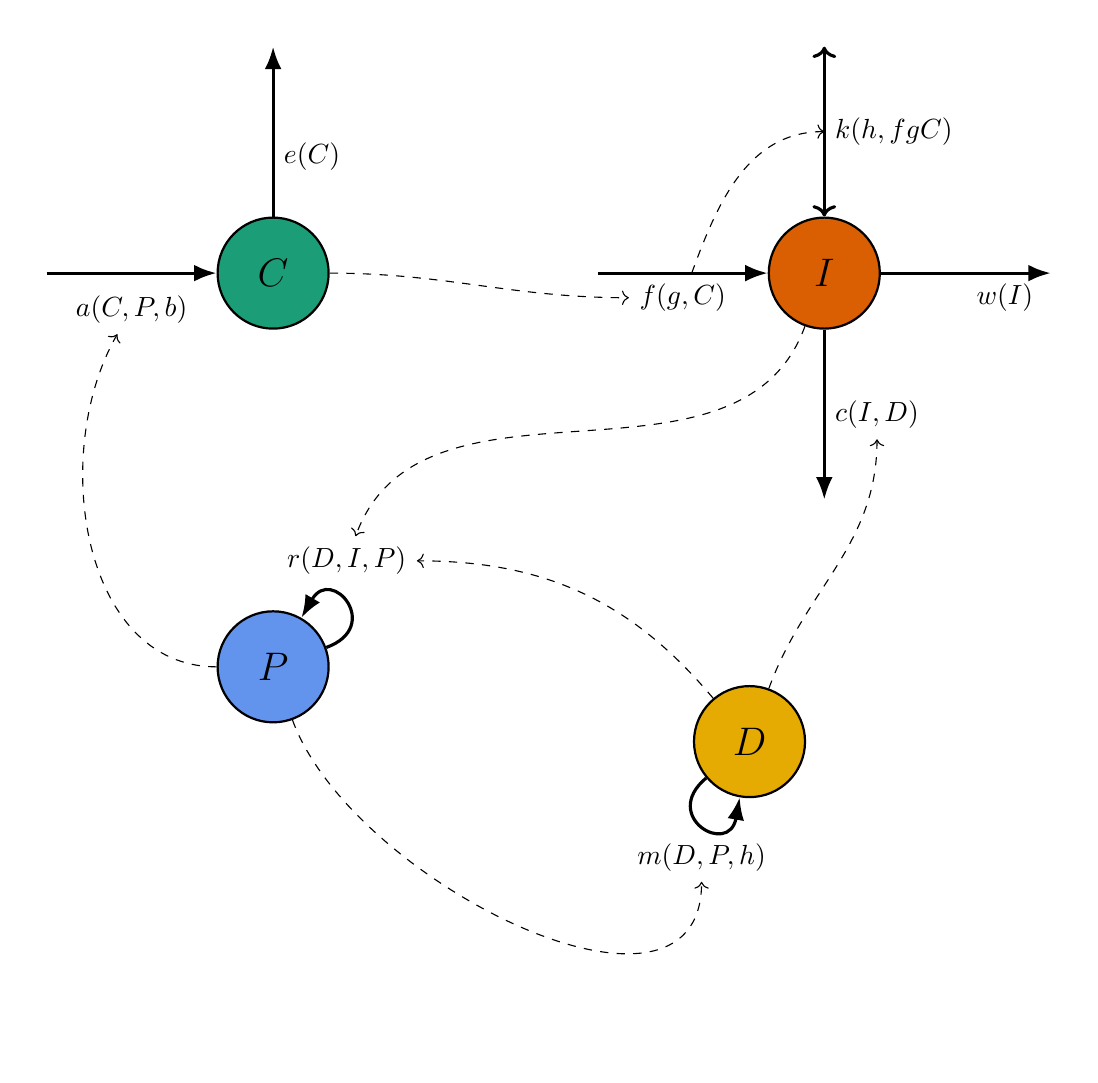
\begin{tikzpicture}[
  ampersand replacement=\&,
  state/.style = {circle, thick, fill=cornflowerblue!30, draw=black, text width = 3em, align=center, node distance = 7cm, font=\Large},
  ph/.style = {node distance = 3cm},
  flow/.style = {-Latex, line width=.4mm},
  flow_lab/.style = {font=\normalfont}
  ]

  \node[state, fill=capitalcolour] (capital) {$C$};
  \node[state, fill=inventorycolour, right of = capital] (inventory) {$I$};
  \node[state, fill=demandcolour, below left of = inventory, xshift=4cm, yshift=-1cm] (demand) {$D$};
  \node[state, fill=cornflowerblue, below of = capital, yshift=2cm] (price) {$P$};

  \node[ph, left of=capital] (capital_in) {};
  \draw[flow] (capital_in) -- node[below=.15cm, flow_lab] (replace) {$a(C, P, b)$} (capital);
  \node[ph, above of = capital] (capital_deprec) {};
  \draw[flow] (capital) -- node[below right,flow_lab] (depreciation) {$e(C)$} (capital_deprec) {};
  \node[ph, left of = inventory] (inventory_in) {};
  \draw[flow] (inventory_in) -- node[below, flow_lab] (d_production) {$f(g, C)$} (inventory) {};
  \draw[dashed,->] (capital) to[out=0,in=180] (d_production);

  \node[ph, right of = inventory] (inventory_waste) {};
  \draw[flow] (inventory) to node[below right, flow_lab] (waste) {$w(I)$} (inventory_waste);
  \node[ph, above of = inventory] (imports) {};
  \draw[flow,<->] (imports) to node[right, flow_lab] (importing) {$k(h,fgC)$} (inventory);
  \draw[dashed,->] (d_production) to[out=70,in=180] (importing);
  \node[ph, below of = inventory] (consumption) {};
  \draw[flow] (inventory) to node[right,flow_lab] (consuming) {$c(I,D)$} (consumption);

  \draw[flow] (demand) to[out=220, in=260, looseness=4] node[flow_lab, below =.1cm] (demand_change) {$m(D, P, h)$} (demand);
  \draw[dashed,->] (demand) to[out=70,in=270] (consuming);

  \draw[flow] (price) to[out=20, in=60, looseness=4] node[flow_lab, above=.25cm] (price_change) {$r(D, I, P)$} (price);
  \draw[dashed,->] (inventory) to[out=250,in=70] (price_change);
  \draw[dashed,->] (demand) to[out=130, in=0] (price_change);
  \draw[dashed,->] (price) to[out=290,in=270] (demand_change);

  \draw[dashed,->] (price) to[out=180, in=240] (replace);

\end{tikzpicture}

\end{document}
